\documentclass[12pt]{article}
\usepackage{amsmath, amssymb}
\usepackage[most]{tcolorbox}
\usepackage{fancyhdr}
\usepackage{graphicx}
\usepackage{lmodern}
\usepackage{xcolor}
\usepackage{enumitem}
\usepackage{amsthm}

\definecolor{color1}{HTML}{941b0c}
\definecolor{color2}{HTML}{bc3908}
\definecolor{color3}{HTML}{f6aa1c}

\usepackage[font=small, labelfont=bf, justification=centering]{caption}
\usepackage[colorlinks=true, linkcolor=black, urlcolor=color2, citecolor=black]{hyperref}
\usepackage[a4paper, margin=1in]{geometry}

\title{\sffamily\bfseries{Soluções TM$^2$ 2024A}}
\author{Samuel de Araújo Brandão}
\date{2 de Agosto de 2025}

\renewcommand*\contentsname{\textsf{Contents}}

\pagestyle{fancy}
\fancyhf{}

\fancyhead[L]{\textbf{Soluções TM$^2$ 2024A}}
\fancyhead[R]{\textcolor{color2}{Samuel Brandão}, 2 de Agosto de 2025}
\fancyfoot[C]{\thepage}
\setlength{\headheight}{14.5pt}

\tcbset{
  problembox/.style = {
    enhanced,
    colback=white,
    colframe=color2,
    boxrule=1pt,
    arc=2mm,
    top=1pt,
    bottom=1pt,
    left=1pt,
    right=1pt,
    fonttitle=\sffamily\bfseries\color{white},
    colbacktitle=color2,
    title={#1}
  }
}

\tcbset{
  claimbox/.style={
    enhanced,
    colback=white,
    colframe=color1,
    boxrule=1pt,
  }
}

\begin{document}
  \maketitle

  Uma coleção de soluções para a TM$^2$ 2024 nível A, inspirada no estilo de Evan Chen.

  Todas as soluções foram inteiramente escritas por mim, enquanto me preparava para a
  International Mathematical Olympiad (IMO).

  Caso encontre algum erro ou tiver sugestões ou comentários, sinta-se a vontade 
  para entrar em contato!

  \tableofcontents
  \clearpage

  \section{\textsf{Problemas}}

  \begin{enumerate}[label=\textbf{\arabic*.}]
    \item Uma \textit{palavra} é uma sequência de letras maiúsculas do
      nosso alfabeto (isto é, há 26 possíveis letras). Uma palavra é chamada de
      \textit{palíndromo} se tem pelo menos duas letras e ela é a mesma palavra se lida da
      esquerda para a direita ou da direita para a esquerda. Por exemplo, as palavras ARARA
      e NOON são palíndromos, mas BOBO e AÑÃ não são palíndromos.

      Dizemos que uma palavra $x$ \textit{contém} uma palavra $y$ se existem letras
      \textit{consecutivas} de $x$ que juntas formam $y$. Por exemplo, a palavra ARARA
      contém a palavra RARA e também a palavra ARARA, mas não contém a palavra ARRA.

      Calcule a quantidade de palavras de 14 letras que contêm algum palíndromo.

    \item Mostre que não existem triplas de inteiros não negativos
      $(x, y, z)$ satisfazendo a equação
      \[
        x^2 = 5^y + 3^z.
      \]

    \item No triângulo escaleno $ABC$, sejam $I$ o seu incentro e $D$ o
      ponto onde $AI$ intersecta $BC$. Sejam $M$ e $N$ os pontos onde o incírculo de $ABC$
      toca $AB$ e $AC$, respectivamente. Seja $F$ o segundo encontro do circuncírculo $(AMN)$
      com o circuncírculo $(ABC)$. Seja $T$ o encontro de $AF$ com o prolongamento de $BC$.
      Seja $J$ a interseção de $TI$ com a paralela a $FI$ que passa por $D$. Prove que $AJ$ é
      perpendicular a $BC$.

      \begin{figure}[h]
        \centering
          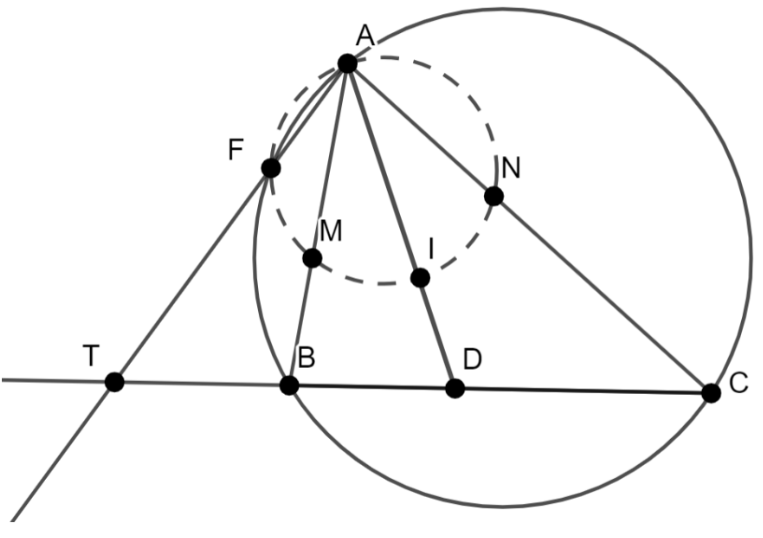
\includegraphics[width=0.5\textwidth]{third.png}
          \caption{Uma ilustração do terceiro problema.}
      \end{figure}

      \textit{Nota: o incentro de um triângulo é a interseção das bissetrizes internas.}

    \item   Encontre todos os inteiros positivos $a$, $b$ e $c$ tais que $3ab = 2c^2$
      e $ a^3 + b^3 + c^3$ seja o dobro de um número primo.
  \end{enumerate}

  \clearpage

  \section{\textsf{Soluções}}
    \subsection{Problema 1.}
      \begin{tcolorbox}[problembox={Enunciado do problema}]
        Uma \textit{palavra} é uma sequência de letras maiúsculas do
        nosso alfabeto (isto é, há 26 possíveis letras). Uma palavra é chamada de
        \textit{palíndromo} se tem pelo menos duas letras e ela é a mesma palavra se lida da
        esquerda para a direita ou da direita para a esquerda. Por exemplo, as palavras ARARA
        e NOON são palíndromos, mas BOBO e AÑÃ não são palíndromos.

        Dizemos que uma palavra $x$ \textit{contém} uma palavra $y$ se existem letras
        \textit{consecutivas} de $x$ que juntas formam $y$. Por exemplo, a palavra ARARA
        contém a palavra RARA e também a palavra ARARA, mas não contém a palavra ARRA.

        Calcule a quantidade de palavras de 14 letras que contêm algum palíndromo.
      \end{tcolorbox}
      Sabe-se que existem \(26^{14}\) possibilidades de palavras de \(14\) letras no total. Além disso, podemos afirmar também que toda palavra contém no mínimo um palíndromo de $2$ ou $3$ letras.
      Isso ocorre porque, ao retirar as primeira e última letras de um palíndromo, será obtido outro palíndromo (caso tenha mais de $2$ letras). É possível repetir isso até chegar
      a $xx$ (um palíndromo de $2$ letras), ou $xyx$ (um palíndromo de $3$ letras).
  
      Existem 26 possíveis letras para a \(1\textsuperscript{a}\) letra de um não palíndromo de 14 totais letras. Afim de evitar um palíndromo, a \(2\textsuperscript{a}\)
      deve ser diferente da \(1\textsuperscript{a}\), (25 opções). Pelo mesmo motivo, a \(3\textsuperscript{a}\) é diferente da \(1\textsuperscript{a}\) e da \(2\textsuperscript{a}\),
      (24 opções). Esse argumento da \(3\textsuperscript{a}\) letra será válido para todas as outras 11 letras. Com isso podemos concluir que existem \(26^{14} - 26 \cdot 25 \cdot 24^{12}\)
      palíndromos no total.
    
    \clearpage

    \subsection{Problema 2.}
      \begin{tcolorbox}[problembox={Enunciado do problema}]
        Mostre que não existem triplas de inteiros não negativos $(x, y, z)$
        satisfazendo a equação
        \[
          x^2 = 5^y + 3^z.
        \]
      \end{tcolorbox}
      Já que \textit{ímpar + ímpar = par}, $5^y + 3^z$ é par, logo $x$ é par. 
      Se $x = 2k$, $x^2 = 4k^2$, logo $x^2 \equiv 0 \pmod{4}$. Neste caso,
      $0 \equiv 5^y + 3^z \equiv 1 + (-1)^z \pmod{4}$, por conseguinte, $z$ é um número
      ímpar. Claramente, $x \not\equiv 0 \pmod{3}$, pois
      \[
        x \equiv 0 \pmod{3} \Rightarrow 5^y = x^2 - 3^z \Rightarrow 5^y \equiv 0 \pmod{3}
      \]
      Absurdo! Agora, nos resta apenas $x \equiv 1 \pmod{3}$ ou $x \equiv 2 \pmod{3}$. Perceba abaixo
      que $x \not\equiv 1 \pmod{3}$ e $x \not\equiv 2 \pmod{3}$, e como já vimos que
      $x \not\equiv 0 \pmod{3}$, não existem soluções para $x$.
      \begin{enumerate}
        \item \textit{Caso 1:} $x \equiv 1 \pmod{3} \Rightarrow x^2 - 5^y = 3^z \Rightarrow y = 2w$. Neste caso, podemos afirmar
          que $x^2 - 5^{2w} = 3^z \Rightarrow (x + 5^w)(x - 5^w) = 3^z$. Para que esta igualdade
          seja verdadeira, ou $x + 5^w \equiv 0 \pmod{3} \quad \text{e} \quad x - 5^w = 1$, ou, tanto
          $x + 5^w$ quanto $x - 5^w$ são múltiplos de 3. Evidentemente $x - 5^w \neq 1$,
          pois se $x - 5^w = 1$, $5^w + 1 \equiv 1 \pmod{3} \Rightarrow 5^w \equiv 0 \pmod{3}$, absurdo!
          Mas é impossível também que tanto $x + 5^w$ quanto $x - 5^w$ sejam múltiplos de 3, pois neste caso,
          $x \equiv 5^w \pmod{3} \Rightarrow  x \equiv 5^w \equiv 1 \pmod{3}$, impossibilitando que
          $x - 5^w \equiv 0 \pmod{3} \therefore x \not\equiv 1 \pmod{n}$

        \item \textit{Caso 2:} $x \equiv 2 \pmod{3} \Rightarrow x^2 \equiv 5^w \equiv 1 \pmod{3}$.
          Evidentemente $x + 5^w \not\equiv 0 \pmod{3}$, logo a única opção é que $x + 5^w = 1$, claramente impossível já
          que tanto $x$ quanto $w$ são números inteiros positivos $\therefore x \not\equiv 2 \pmod{3}$
  \end{enumerate}

    \clearpage

        \subsection{Problema 3.}
      \begin{tcolorbox}[problembox={Enunciado do problema}]
        No triângulo escaleno $ABC$, sejam $I$ o seu incentro e $D$ o ponto onde $AI$
        intersecta $BC$. Sejam $M$ e $N$ os pontos onde o incírculo de $ABC$ toca $AB$
        e $AC$, respectivamente. Seja $F$ o segundo encontro do circuncírculo $(AMN)$
        com o circuncírculo $(ABC)$. Seja $T$ o encontro de $AF$ com o prolongamento
        de $BC$. Seja $J$ a interseção de $TI$ com a paralela a $FI$ que passa por $D$.
        Prove que $AJ$ é perpendicular a $BC$.

        \centering
          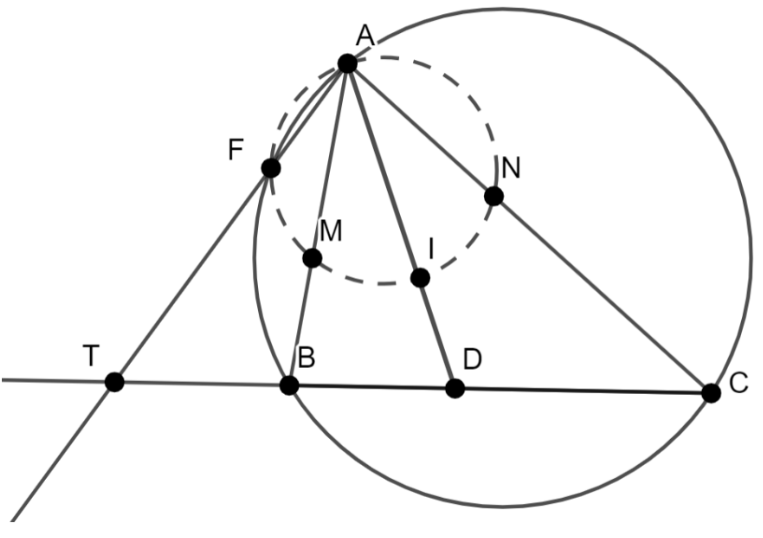
\includegraphics[width=0.5\textwidth]{third.png}

        \textit{Nota: o incentro de um triângulo é a interseção das bissetrizes internas.}
      \end{tcolorbox}

      \begin{figure}[h]
        \centering
        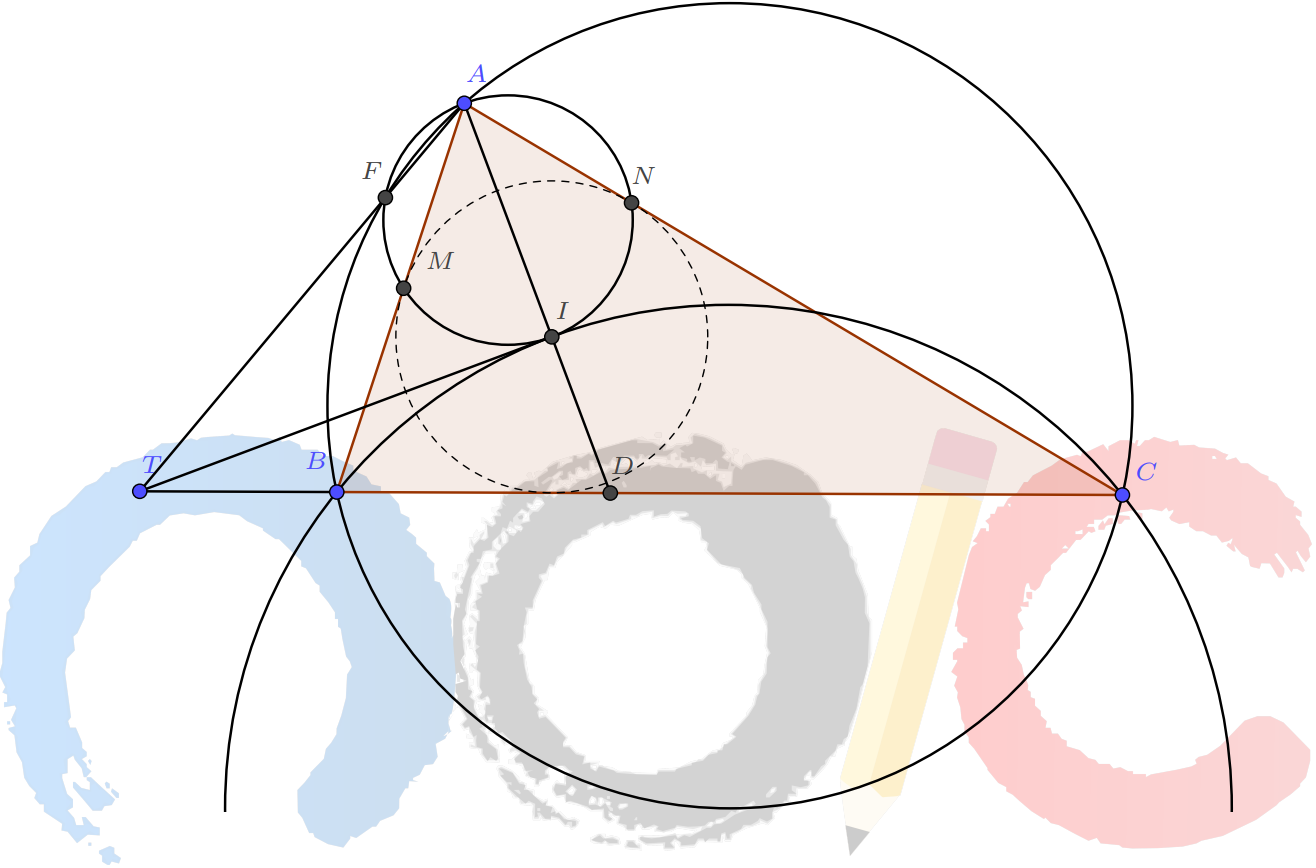
\includegraphics[width=0.5\textwidth]{fourth.png}
        \caption{Uma figura ilustrando a solução para o terceiro problema. \href{https://noic.com.br/wp-content/uploads/2025/03/Solucoes_do_TM2_2024_Nivel_A.pdf}{Fonte.}}
      \end{figure}

      $\overline{AI}$ é um diâmetro de (AMN), pois $\overline{AB}$ é tangente a (MND), logo
      $\angle{AMI} = 90^{\circ}$. Por conseguinte, $\angle{AIT} = 90^{\circ}$ resulta em
      $\angle AJ'J = 90^{\circ}$, quando J' é a projeção de $\overline{AJ}$ sobre o segmento 
      $\overline{BC}$. Logo, basta provar que $\overline{TI}$ é tangente a (AMN), o que
      resultaria em $\angle{AIT} = 90^{\circ}$.

      \begin{tcolorbox}[claimbox={Claim}]
        \textbf{\sffamily\textcolor{color1}{Alegação ---}} $\overline{TI}$ é tangente às circunferências
        $(AMN)$ e $(BIC)$.
      \end{tcolorbox}

      \textit{Prova.} Já que $T \in \overline{AF}, \overline{BC}$, justamente o \textit{Eixo Radical}
      de, respectivamente, $(AMN)$, $(ABC)$ e $(ABC)$, $(BIC)$, pode-se afirmar que $T$ é o \textit{Centro
      Radical} das circunferências $(ABC)$, $(AMN)$ e $(BIC)$.

      Seja $M$ o ponto médio do arco $\overset{\frown}{BC}$, pelo \textit{Lema do Incentro-Excentro}, $M$
      é o centro da circunferência $(BIC)$. O centro das circunferências $(AMN)$ e $(BIC)$ estão ambas sobre
      a reta $\overline{AI}$. Para que isso seja possível, $(AMN)$ e $(BIC)$ devem ser tangentes em $I$. Já
      que $T$ é o \textit{Centro Radical}, $\overline{TI}$ é tangente à $(AMN)$, logo $\angle AJC = 90^{\circ}$. \qed

      \clearpage
    
    \subsection{Problema 4.}
      \begin{tcolorbox}[problembox={Enunciado do problema}]
        Encontre todos os inteiros positivos $a$, $b$ e $c$ tais que $3ab = 2c^2$
        e $ a^3 + b^3 + c^3$ seja o dobro de um número primo.
      \end{tcolorbox}

  \clearpage
  
  \section{\textsf{Referências}}
  Só foi possível escrever este documento graças a ajuda e inspiração dos seguintes:

  \renewcommand{\refname}{\vspace{-2em}}
  \begin{thebibliography}{9}
    \bibitem{noic}
    NOIC - Núcleo Olímpico de Iniciação Científica.
    \textit{Soluções do TM$^2$ Nível A}, 2025.
    Disponível em: \url{https://noic.com.br/wp-content/uploads/2025/03/Solucoes_do_TM2_2024_Nivel_A.pdf}
  \end{thebibliography}
\end{document}
